%Classification ascendante hiérarchique

\subsubsection{Démarche}

La démarche pour les deux méthodes consiste à appliquer respectivement une ACP, après normalisation, et une ACM aux données, après mise en classe, puis de classer les résultats par une méthode de Classification ascendante hiérarchique (CAH).

Les données utilisées dans l'exemple donné en graphique sont issues de la base "populations".

Ces données étant quantitatives, l'ACP peut s'appliquer directement, mais il faut réaliser une mise en classe pour obtenir un tableau disjonctif complet (TDC) et réaliser l'ACM. L'ACM correspont à une Analyse factoriel des correspondances binaires (AFC) d'un TDC, qui n'est pas traité dans ce rapport.

En suite, on utilise la méthode de Classification ascendante hiérarchique (CAH). Tout d'abord, on réalise la construction de l'arbre hiérarchique par agrégations successives de deux éléments en utilisant la fonction \textit{linkage} issue du module \textit{scipy.cluster.hierarchy (Hierarchical clustering)}. Cette fonction admet différentes méthodes pour calculer la distance entre des éléments (cf. Figure \ref{fig: Label methodes_linkage.jpg}):

%------ Pour insérer et citer une image centralisée -----
\insererfigure{img/methodes_linkage.jpg}{11.5cm}{Méthodes pour la fonction linkage : single, complete, average, centroid, median et ward. \\ Source : ScyPy.org }{Label methodes_linkage.jpg}
% Le premier argument est le chemin pour la photo
% Le deuxième est la hauteur de la photo
% Le troisième la légende
% Le quatrième le label)

L'affichage de l'arbre hiérarchique par agrégations successives grâce à un dendrogram (fonction \textit{dendrogram} du module \textit{scipy.cluster.hierarchy (Hierarchical clustering)}). 

La coupure de l'arbre hiérarchique pour obtenir une partition est effectué ensuite avec la fonction \textit{fcluster} du même module. La partition obtenu aide aussi à représenter graphiquement le résultat, en affichant les points avec un colleur diffèrent en fonction de la partition à laquelle l'élément fait partie.

Pour l'ACP :

\begin{figure}[!htb]
        %\captionsetup[subfigure]{labelformat=empty}
        \begin{subfigure}[b]{1.0\textwidth}
            \centering
            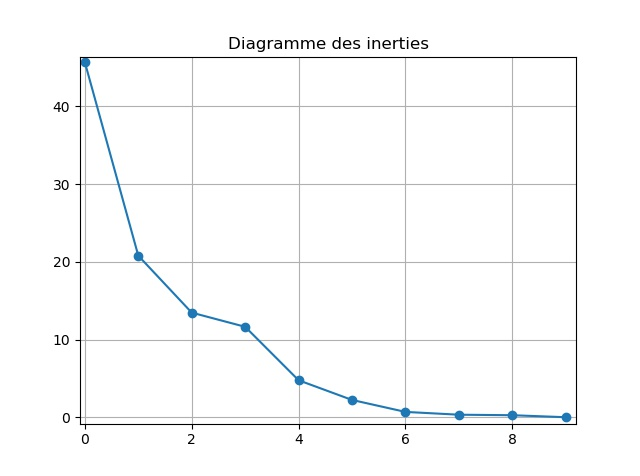
\includegraphics[width=0.6\textwidth]{img/mixte_acp_cah/diagramme_des_inerties.jpg}
            \caption{ACP : Diagramme des inerties}
            \label{Label_diagramme_des_inerties.jpg}
        \end{subfigure}\\
        
        \begin{subfigure}[b]{1.0\textwidth}
            \centering
            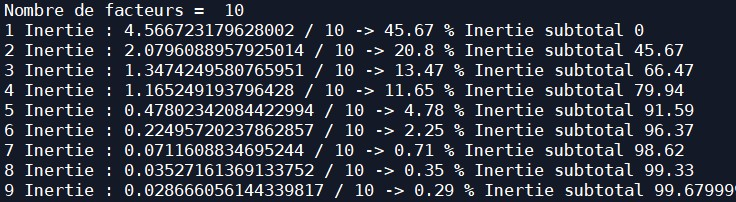
\includegraphics[width=1.0\textwidth]{img/mixte_acp_cah/inerties_acp.jpg}
            \caption{ACP : Inerties de 1 à 9}
            \label{Label_inerties_acp.jpg}
        \end{subfigure}
        \caption{Résultats pour l'ACP}
        \label{Label_inerties}
    \end{figure}
    
    Comme on a une ACP normée, l’inertie totale de chacun des nuages (lignes et colonnes) est égale au nombre de variables actives (ici 10). On peut remarque que le deux premiers facteurs contiennent la majorité $66,47\%$ de l'inertie totale. 
    
    Dans le code du fichier $mixte\_acp\_cah.py$ on réalise un boucle pour prendre des facteurs jusqu'à avoir une pourcentage d'inertie supérieur à $95\%$ pour obtenir une meilleure représentation. Pour le jeu de données \textbf{population}, cela correspond à prendre $6$ facteurs. Ces facteurs totalisent $96,37\%$ de l'inertie totale.
    
    \begin{figure}[!htb]
        %\captionsetup[subfigure]{labelformat=empty}
        \begin{subfigure}[b]{1.0\textwidth}
            \centering
            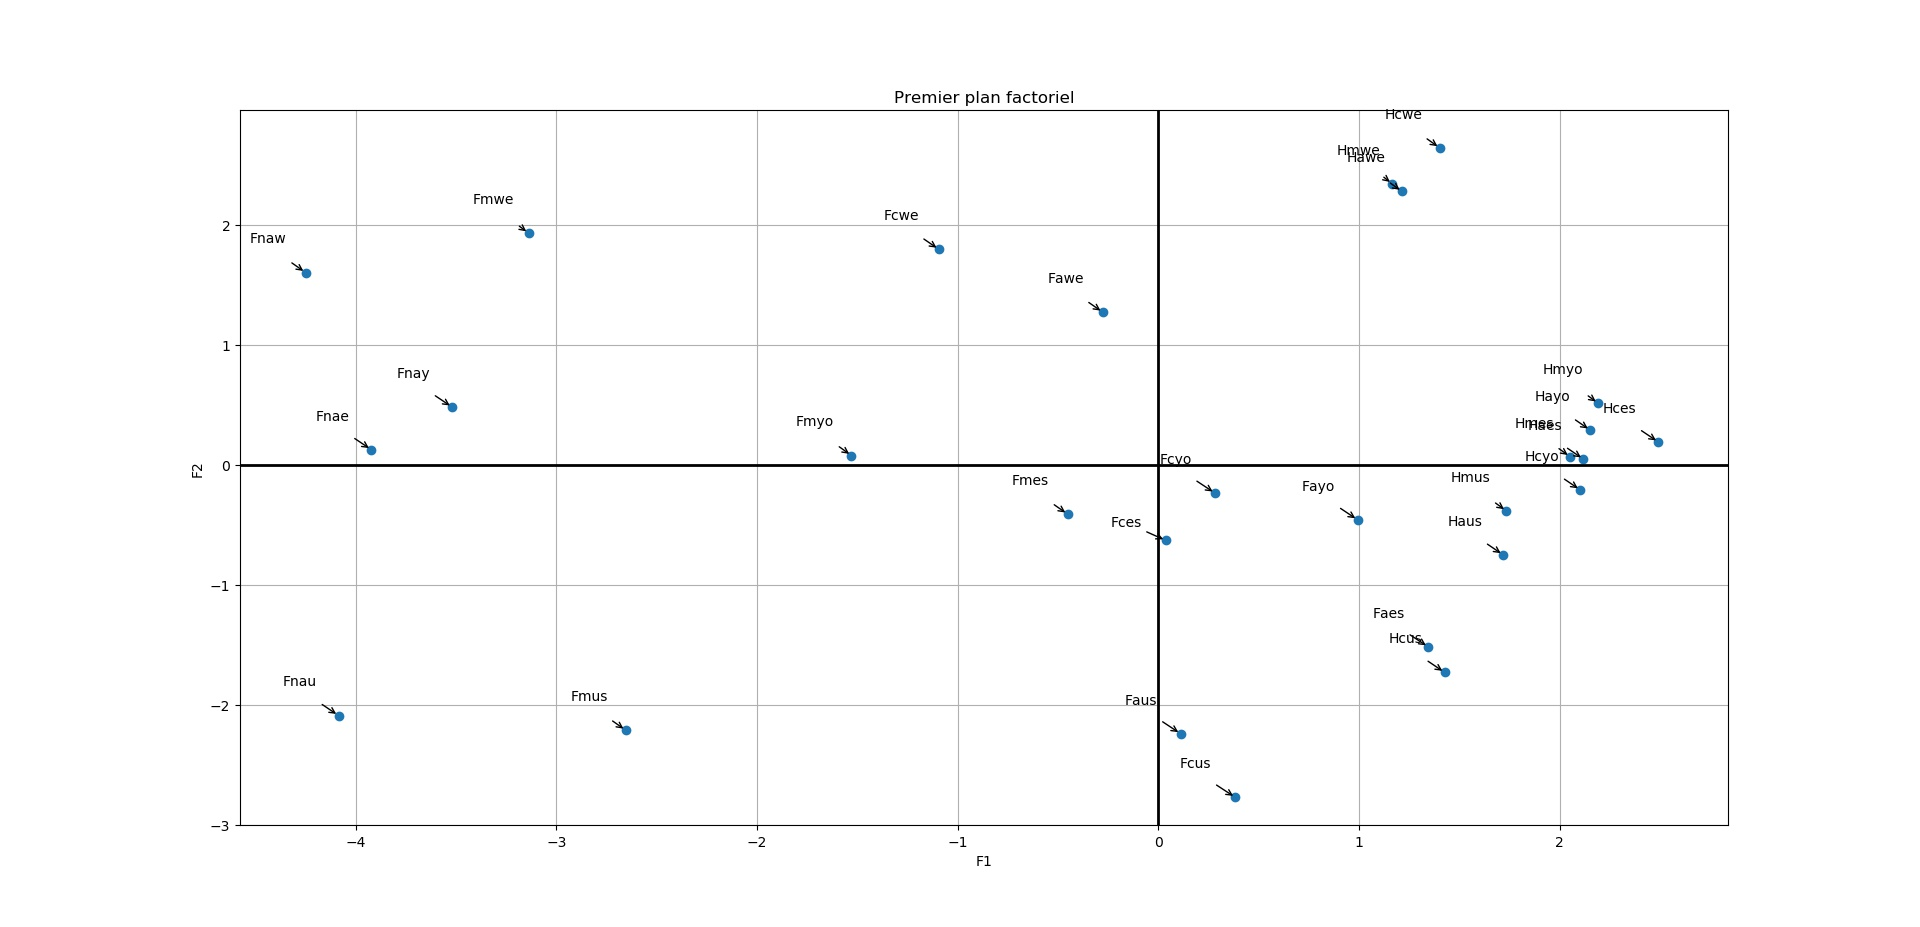
\includegraphics[width=1.0\textwidth]{img/mixte_acp_cah/Projection_des_individus_dans_le_premier_plan_factoriel.jpg}
            \caption{ACP : Projection des individus dans le premier plan factoriel}
            \label{Label_Projection_des_individus_dans_le_premier_plan_factoriel.jpg}
        \end{subfigure}
        \\
        \begin{subfigure}[b]{1.0\textwidth}
            \centering
            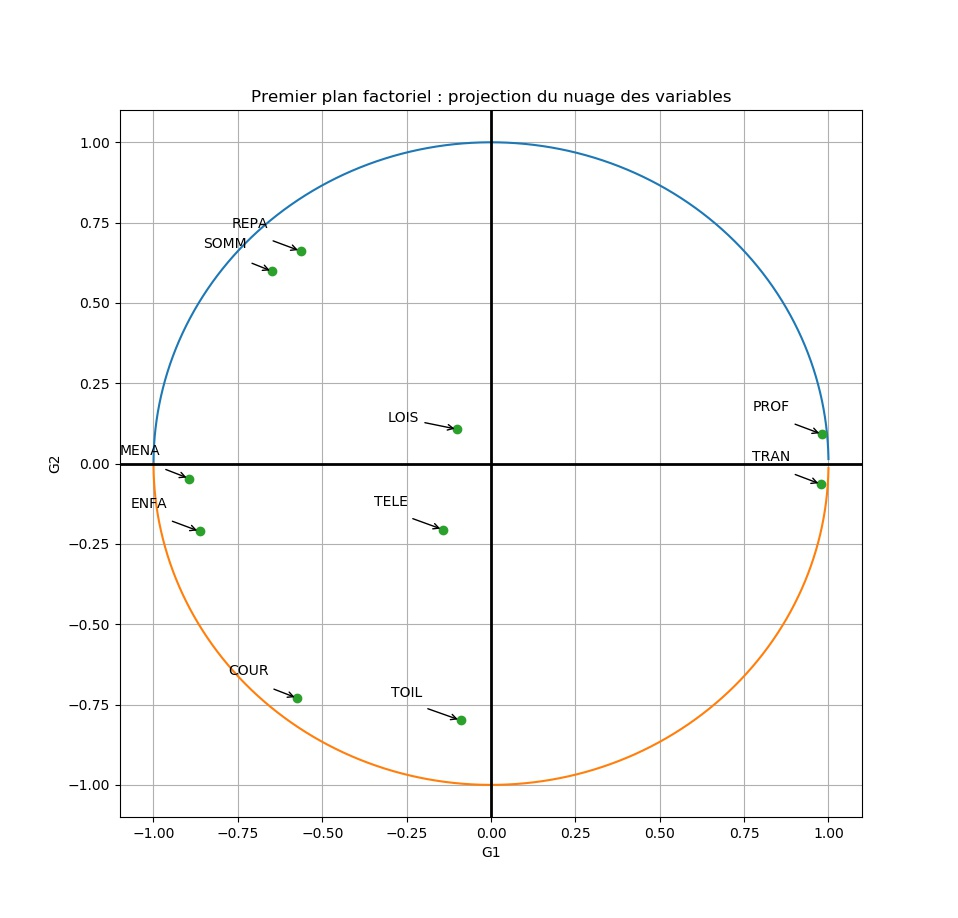
\includegraphics[width=0.6\textwidth]{img/mixte_acp_cah/Projection_du_nuage_des_variables_dans_le_premier_plan_factoriel.jpg}
            \caption{ACP : Projection du nuage des variables dans le premier plan factoriel}
            \label{Label_Projection_du_nuage_des_variables_dans_le_premier_plan_factoriel_acp.jpg}
        \end{subfigure}
        \caption{Projection dans le premier plan factoriel pour l'ACP : individus et variables}
        \label{Label_ACP_Projection_Individus_Variables}
    \end{figure}
    
    Les projections des individus et des variables dans le premier plan factoriel sont montrées dans le Figure \ref{fig: Label_ACP_Projection_Individus_Variables}. 
    
    Les résultats de la CAH sont affichés ci-dessous. On remarque le fait qu'elle mettre en évidence des classes, mais qui cela a une influence de la méthode choisi.
    
    Pour les individus :
    
    \begin{figure}[!htb]
        %\captionsetup[subfigure]{labelformat=empty}
        \begin{subfigure}[b]{1.0\textwidth}
            \centering
            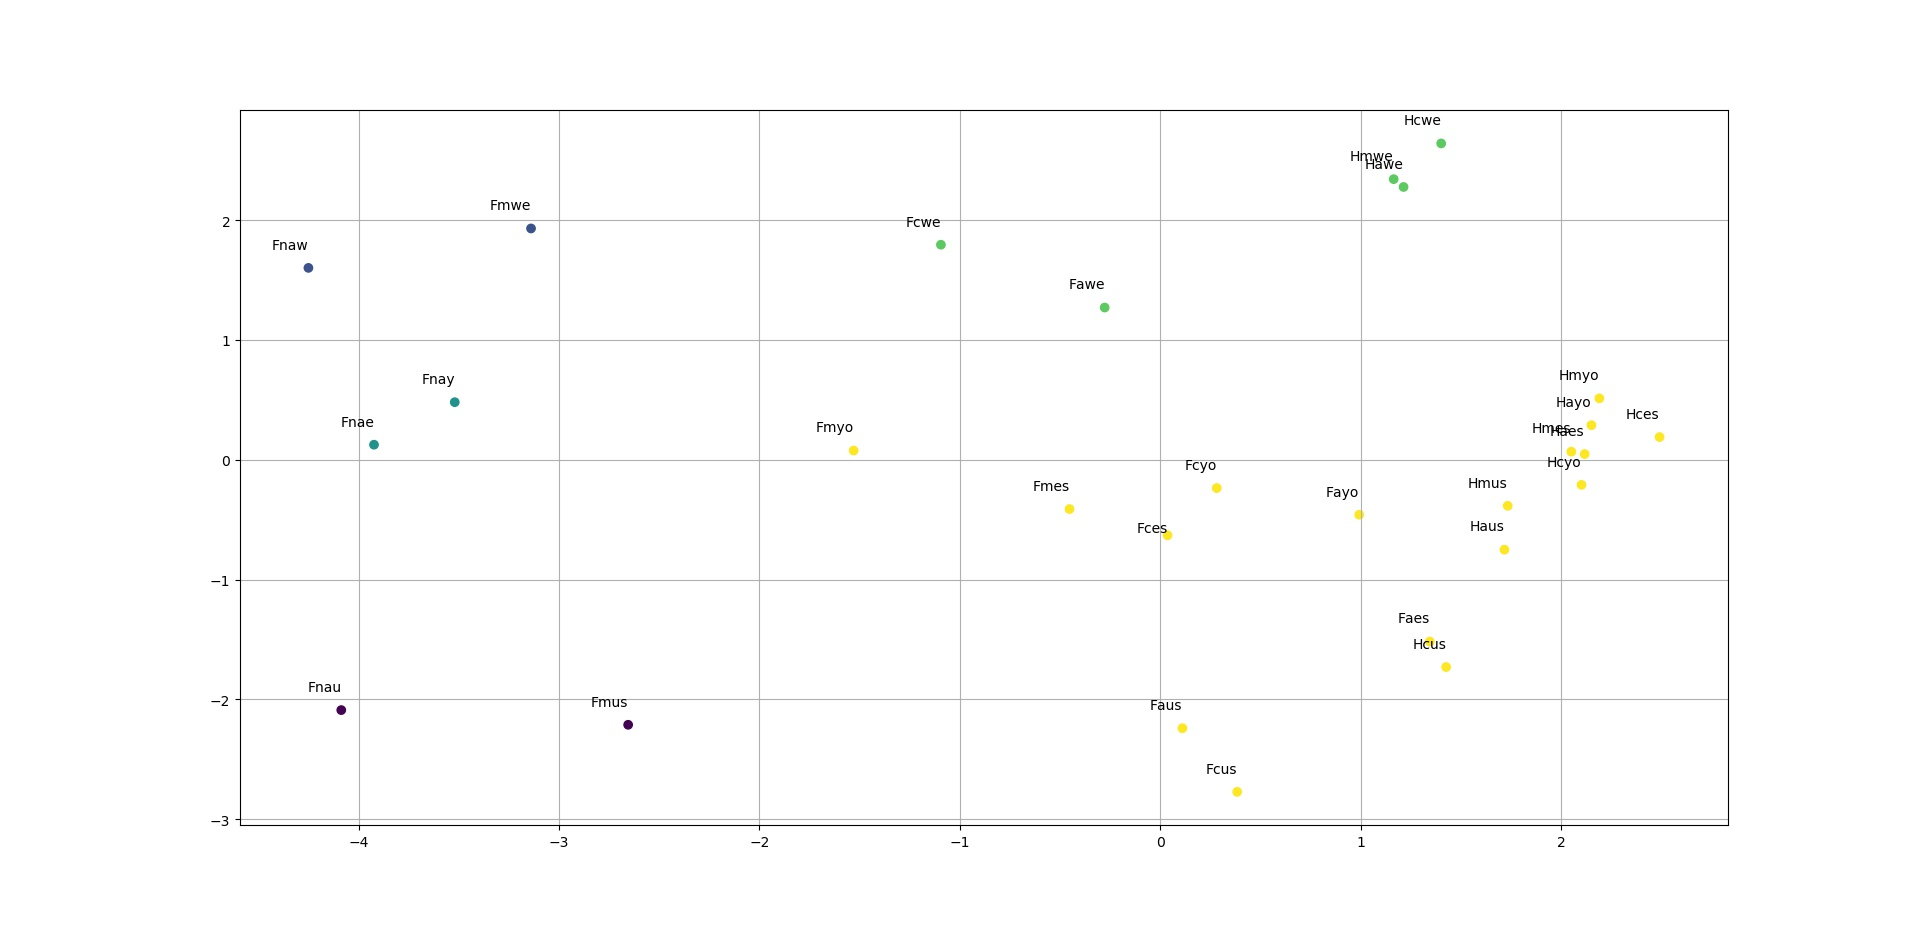
\includegraphics[width=0.95\textwidth]{img/mixte_acp_cah/Projection_des_individus_dans_le_premier_plan_factoriel_cah_'single'_'maxclust'.jpg}
            \caption{ACP + CAH (méthodes single (linkage) et maxclust (fcluster))}
            \label{Label_Projection_des_individus_dans_le_premier_plan_factoriel_cah_'single'_'maxclust'.jpg}
        \end{subfigure}
        \\
        \begin{subfigure}[b]{1.0\textwidth}
            \centering
            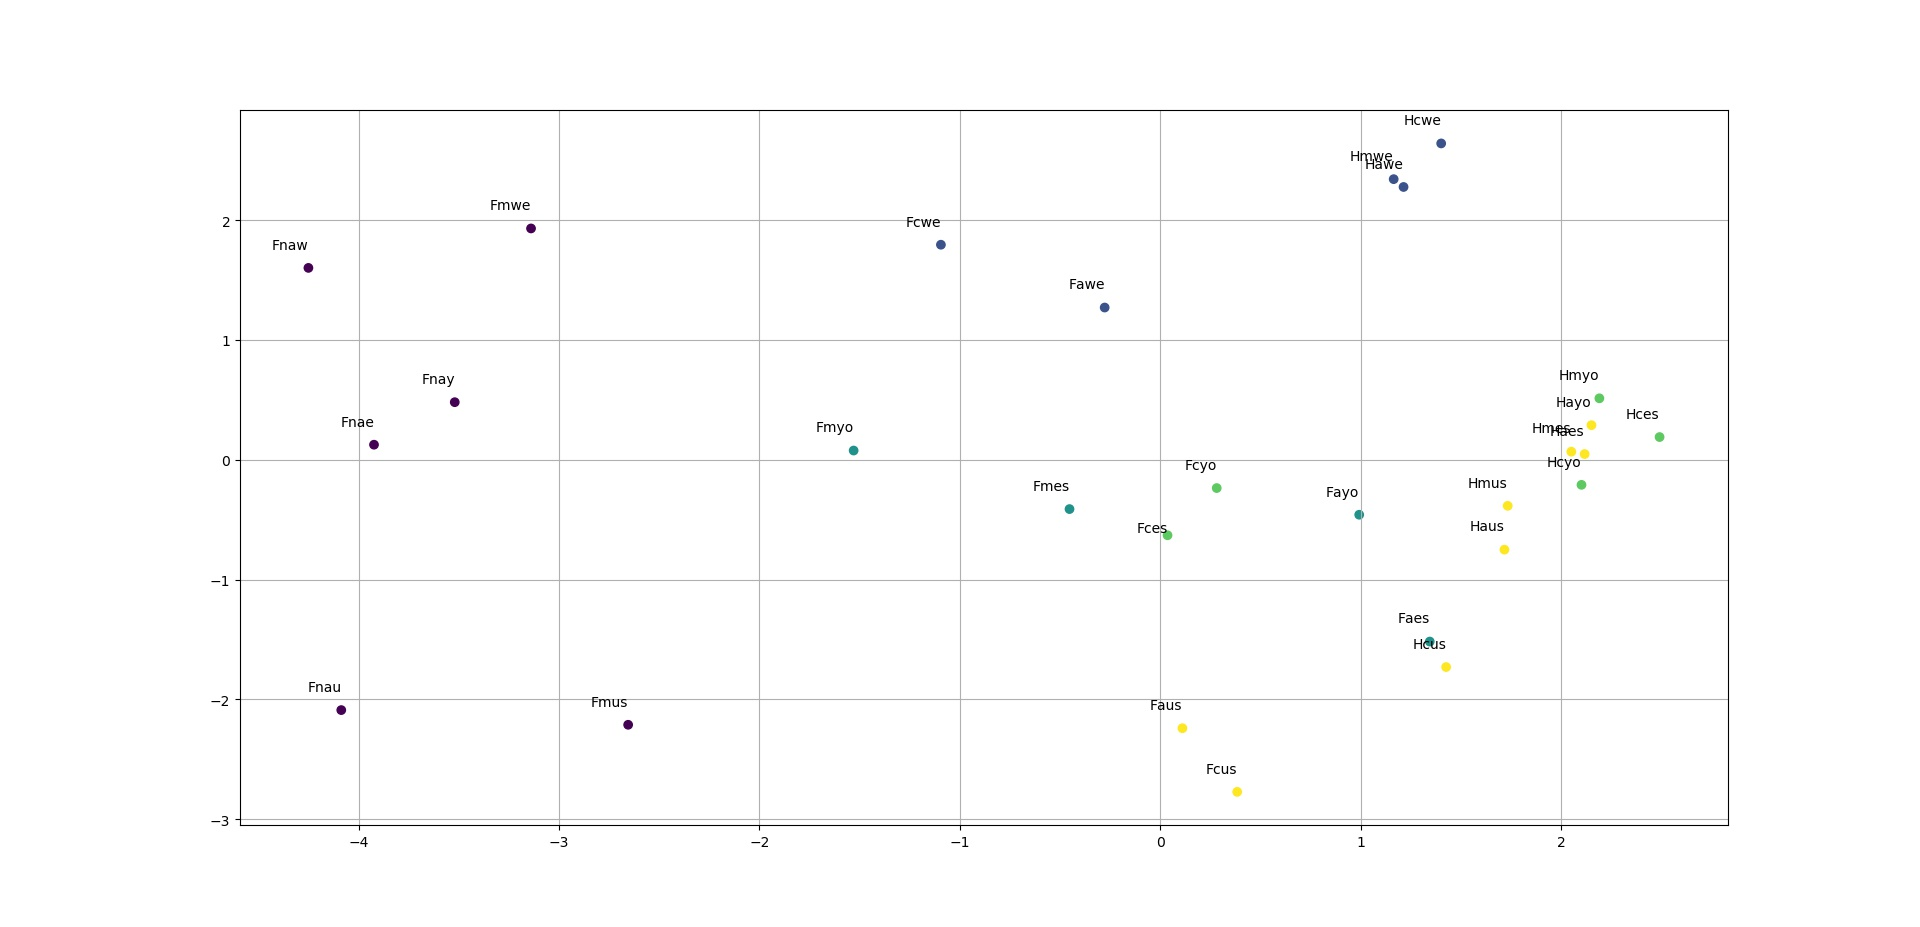
\includegraphics[width=0.95\textwidth]{img/mixte_acp_cah/Projection_des_individus_dans_le_premier_plan_factoriel_cah_'ward'_'maxclust'.jpg}
            \caption{ACP + CAH (méthodes ward (linkage) et maxclust (fcluster))}
            \label{Label_Projection_des_individus_dans_le_premier_plan_factoriel_cah_'ward'_'maxclust'.jpg}
        \end{subfigure}
        \caption{Comparaison ACP + CAH : single x ward pour les individus}
        % \label{Label_ACP_Projection_Individus_Variables.png}
    \end{figure}
    
    \begin{figure}[!htb]
        %\captionsetup[subfigure]{labelformat=empty}
        \begin{subfigure}[b]{1.0\textwidth}
            \centering
            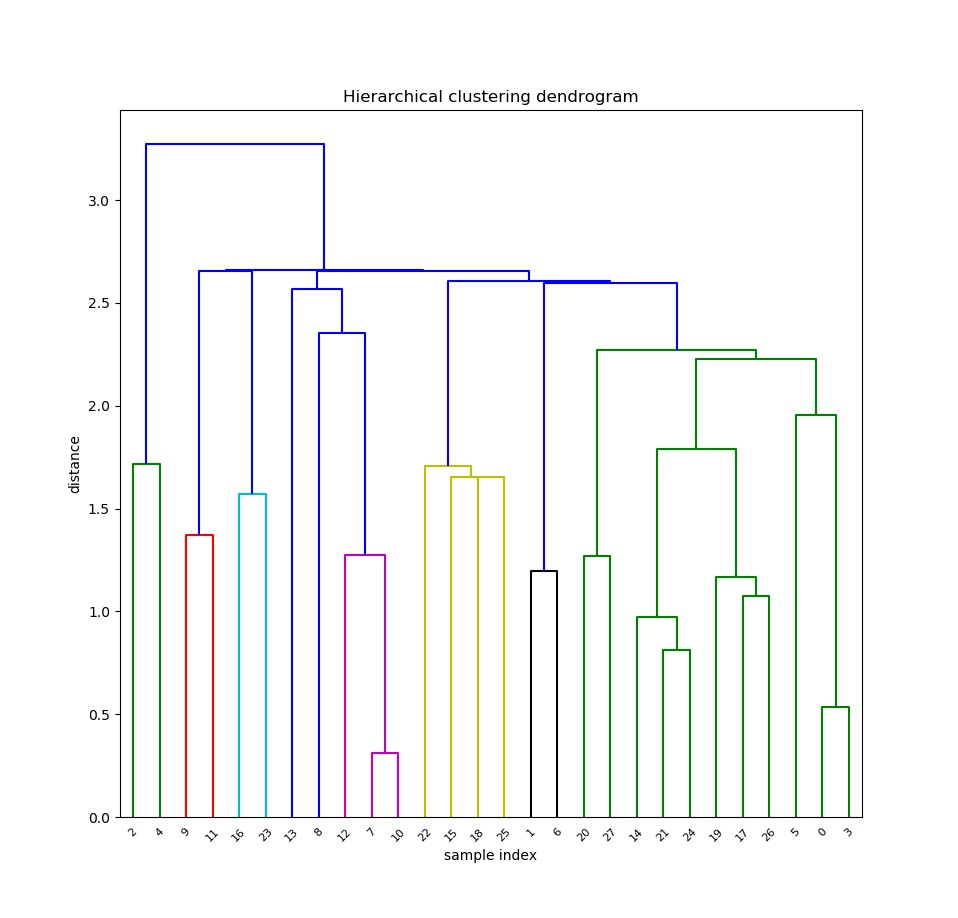
\includegraphics[width=0.7\textwidth]{img/mixte_acp_cah/Dendrogram_individus_'single'_'maxclust'.jpg}
            \caption{Individus : ACP + CAH (méthodes single (linkage) et maxclust (fcluster))}
            \label{Label_Dendrogram_individus_'single'_'maxclust'.jpg}
        \end{subfigure}
        \\
        \begin{subfigure}[b]{1.0\textwidth}
            \centering
            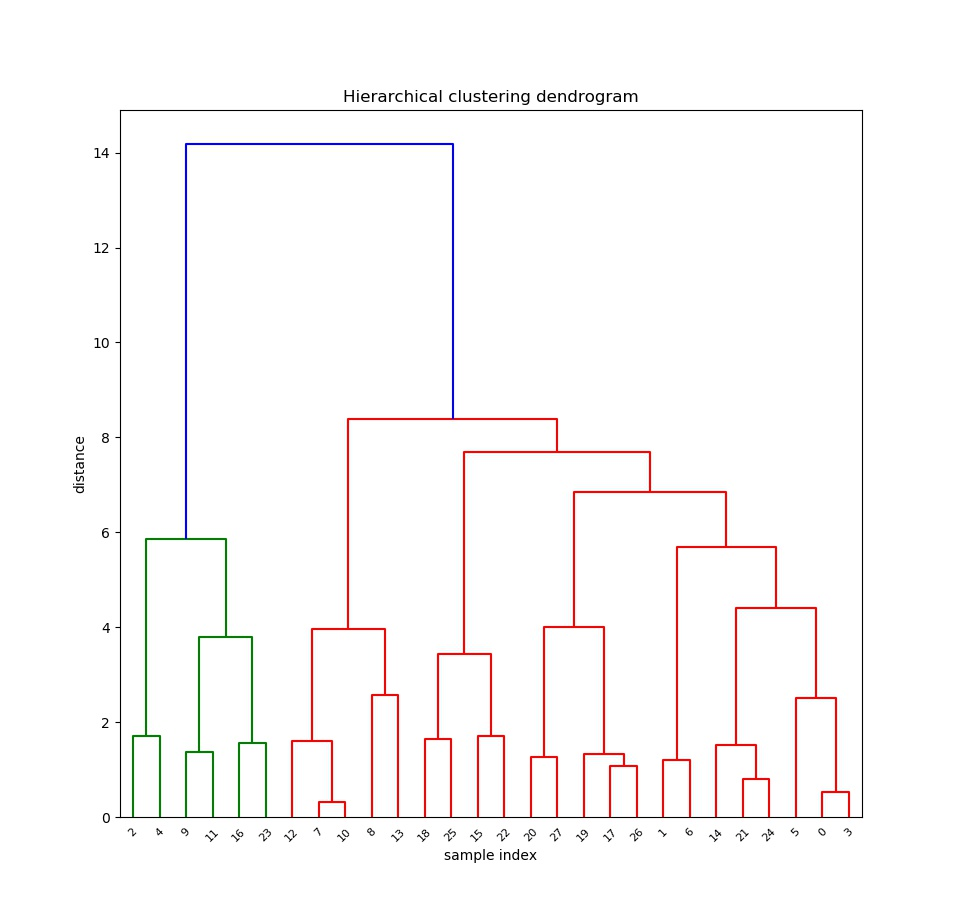
\includegraphics[width=0.7\textwidth]{img/mixte_acp_cah/Dendrogram_individus_'ward'_'maxclust'.jpg}
            \caption{Individus : ACP + CAH (méthodes ward (linkage) et maxclust (fcluster))}
            \label{Label_Dendrogram_individus_'ward'_'maxclust'.jpg}
        \end{subfigure}
        \caption{Comparaison Dendrograms ACP + CAH : single x ward pour les individus}
        % \label{Label_ACP_Projection_Individus_Variables.png}
    \end{figure}
    
    Pour les variables :
    
    \begin{figure}[!htb]
        %\captionsetup[subfigure]{labelformat=empty}
        \begin{subfigure}[b]{1.0\textwidth}
            \centering
            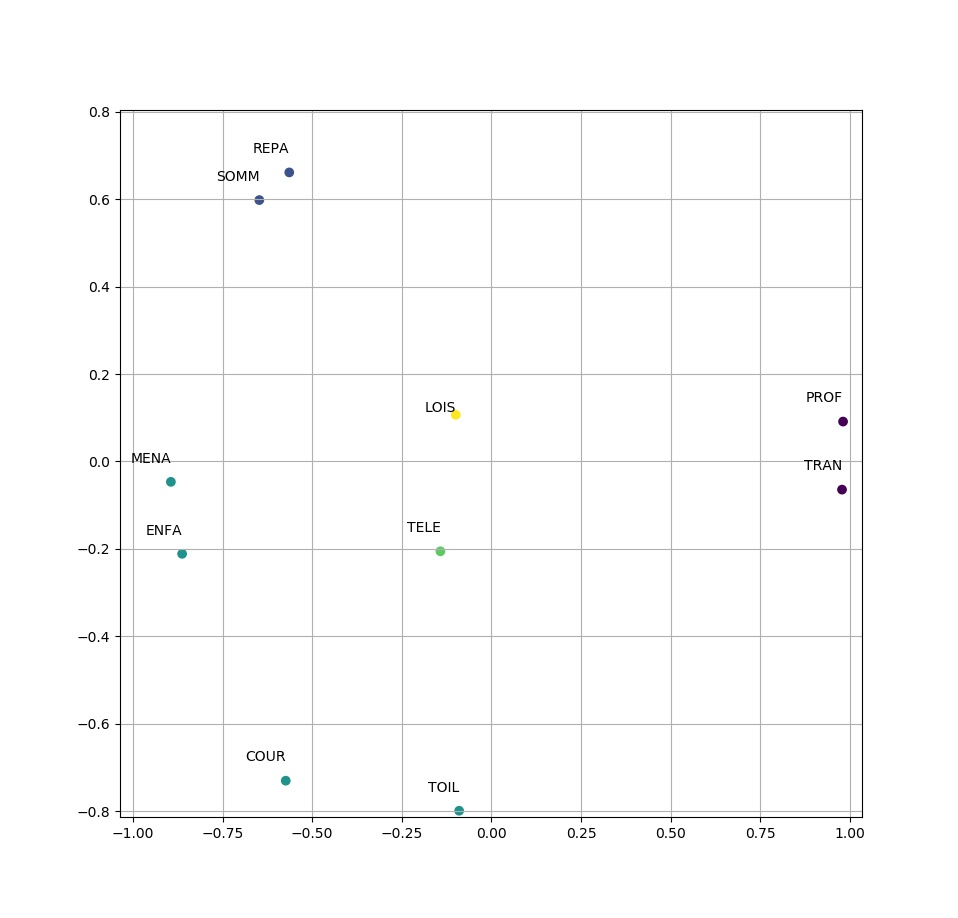
\includegraphics[width=0.71\textwidth]{img/mixte_acp_cah/Projection_du_nuage_des_variables_dans_le_premier_plan_factoriel_cah_'single'_'maxclust'.jpg}
            \caption{Variables : ACP + CAH (méthodes single (linkage) et maxclust (fcluster))}
            \label{Label_Projection_du_nuage_des_variables_dans_le_premier_plan_factoriel_cah_'single'_'maxclust'.jpg}
        \end{subfigure}
        \\
        \begin{subfigure}[b]{1.0\textwidth}
            \centering
            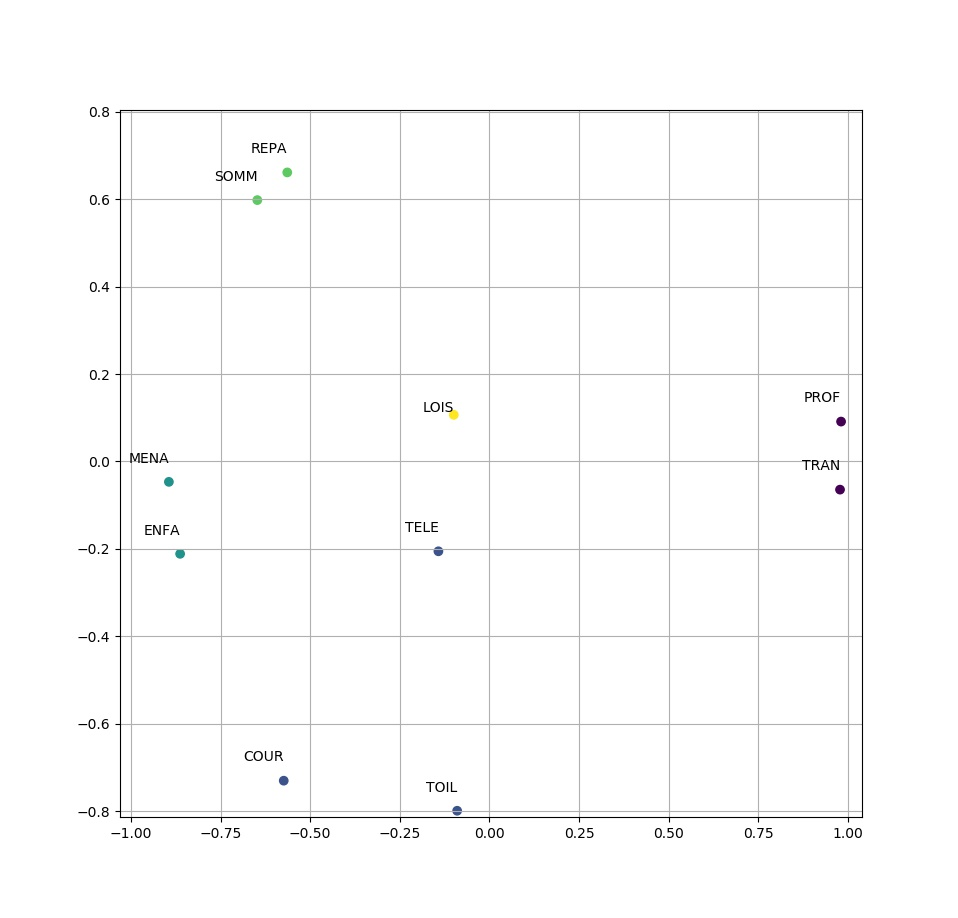
\includegraphics[width=0.71\textwidth]{img/mixte_acp_cah/Projection_du_nuage_des_variables_dans_le_premier_plan_factoriel_cah_'ward'_'maxclust'.jpg}
            \caption{Variables : ACP + CAH (méthodes ward (linkage) et maxclust (fcluster))}
            \label{Label_Projection_du_nuage_des_variables_dans_le_premier_plan_factoriel__cah_'ward'_'maxclust'.jpg}
        \end{subfigure}
        \caption{Comparaison ACP + CAH : single x ward pour les individus}
        % \label{Label_ACP_Projection_Individus_Variables.png}
    \end{figure}
    
    \begin{figure}[!htb]
        %\captionsetup[subfigure]{labelformat=empty}
        \begin{subfigure}[b]{1.0\textwidth}
            \centering
            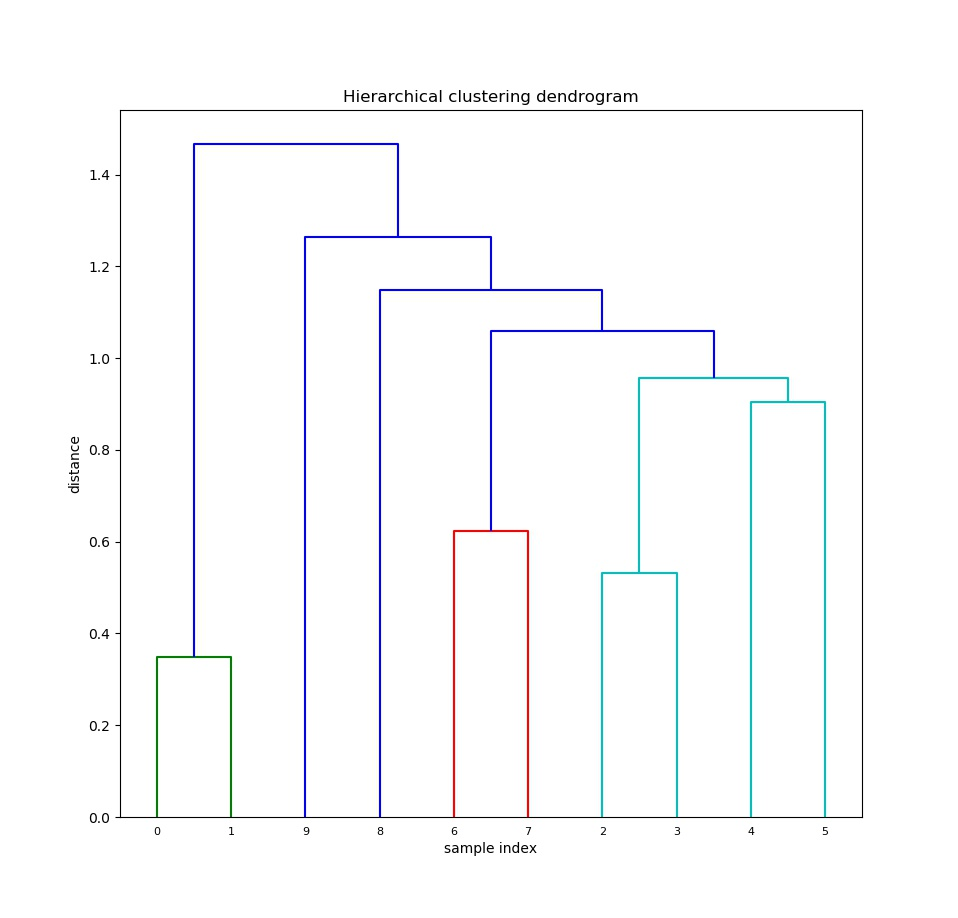
\includegraphics[width=0.7\textwidth]{img/mixte_acp_cah/Dendrogram_variables_'single'_'maxclust'.jpg}
            \caption{Variables : ACP + CAH (méthodes single (linkage) et maxclust (fcluster))}
            \label{Label_Dendrogram_variables_'single'_'maxclust'.jpg}
        \end{subfigure}
        \\
        \begin{subfigure}[b]{1.0\textwidth}
            \centering
            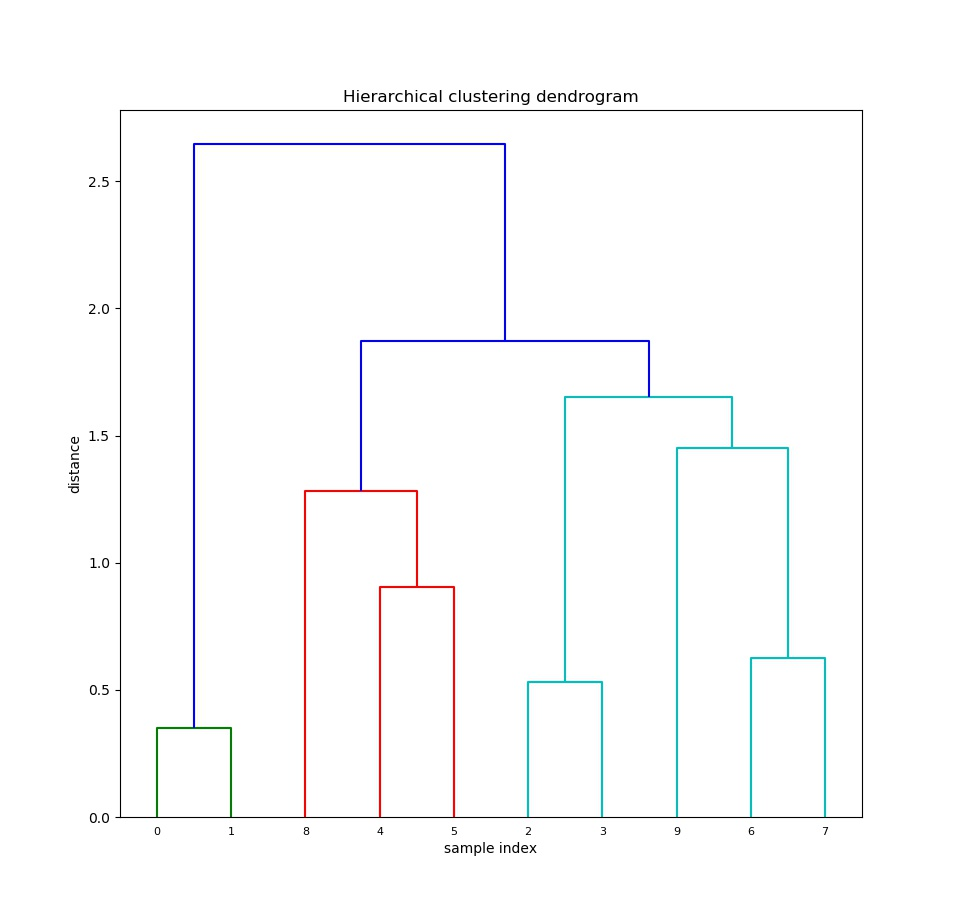
\includegraphics[width=0.7\textwidth]{img/mixte_acp_cah/Dendrogram_variables_'ward'_'maxclust'.jpg}
            \caption{Variables : ACP + CAH (méthodes ward (linkage) et maxclust (fcluster))}
            \label{Label_Dendrogram_variables_'ward'_'maxclust'.jpg}
        \end{subfigure}
        \caption{Comparaison Dendrograms ACP + CAH : single x ward pour les variables}
        % \label{Label_ACP_Projection_Individus_Variables.png}
    \end{figure}
    

Dans les exemples de résultats ci-dessous, on a choisi respectivement un nombre de classes $nClasses = 4$ pour l'ACM.

Pour l'ACM :

\begin{figure}[!htb]
        %\captionsetup[subfigure]{labelformat=empty}
        \begin{subfigure}[b]{1.0\textwidth}
            \centering
            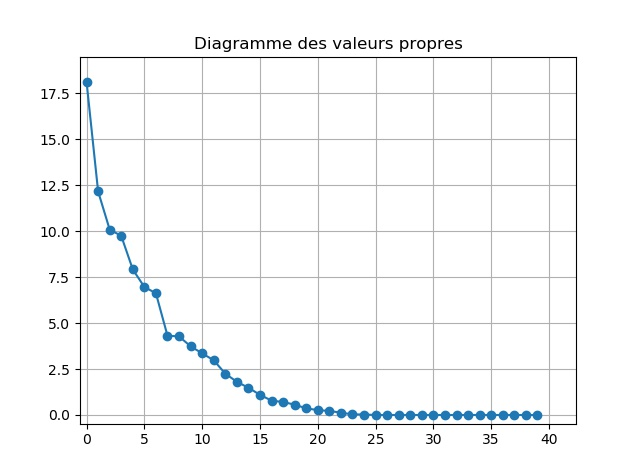
\includegraphics[width=0.6\textwidth]{img/mixte_acm_cah/diagramme_des_valeurs_propres.jpg}
            \caption{ACM : Diagramme des valeurs propres}
            \label{Label_diagramme_des_valeurs_propres.jpg}
        \end{subfigure}
        \\
        \begin{subfigure}[b]{1.0\textwidth}
            \centering
            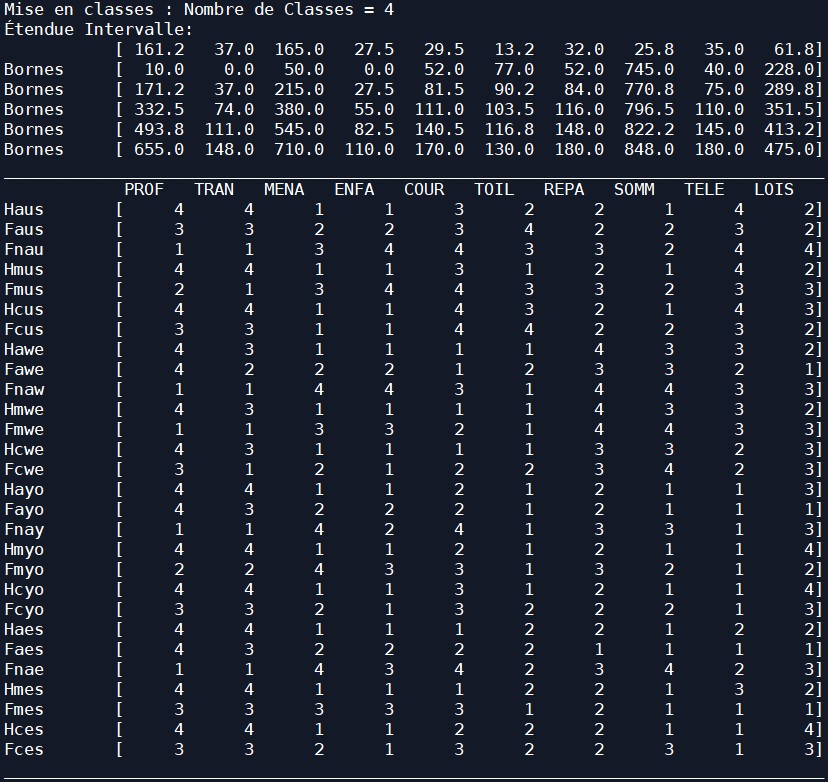
\includegraphics[width=0.9\textwidth]{img/mixte_acm_cah/mise_en_classe_4.jpg}
            \caption{ACM : Mise en classe. Nombre de classes = 4}
            \label{Label_mise_en_classe_4.jpg}
        \end{subfigure}
        \caption{Résultats pour l'ACM}
        %\label{Label_inerties_et_mise_en_classe}
    \end{figure}
    
    \begin{figure}[!htb]
        %\captionsetup[subfigure]{labelformat=empty}
        \begin{subfigure}[b]{1.0\textwidth}
            \centering
            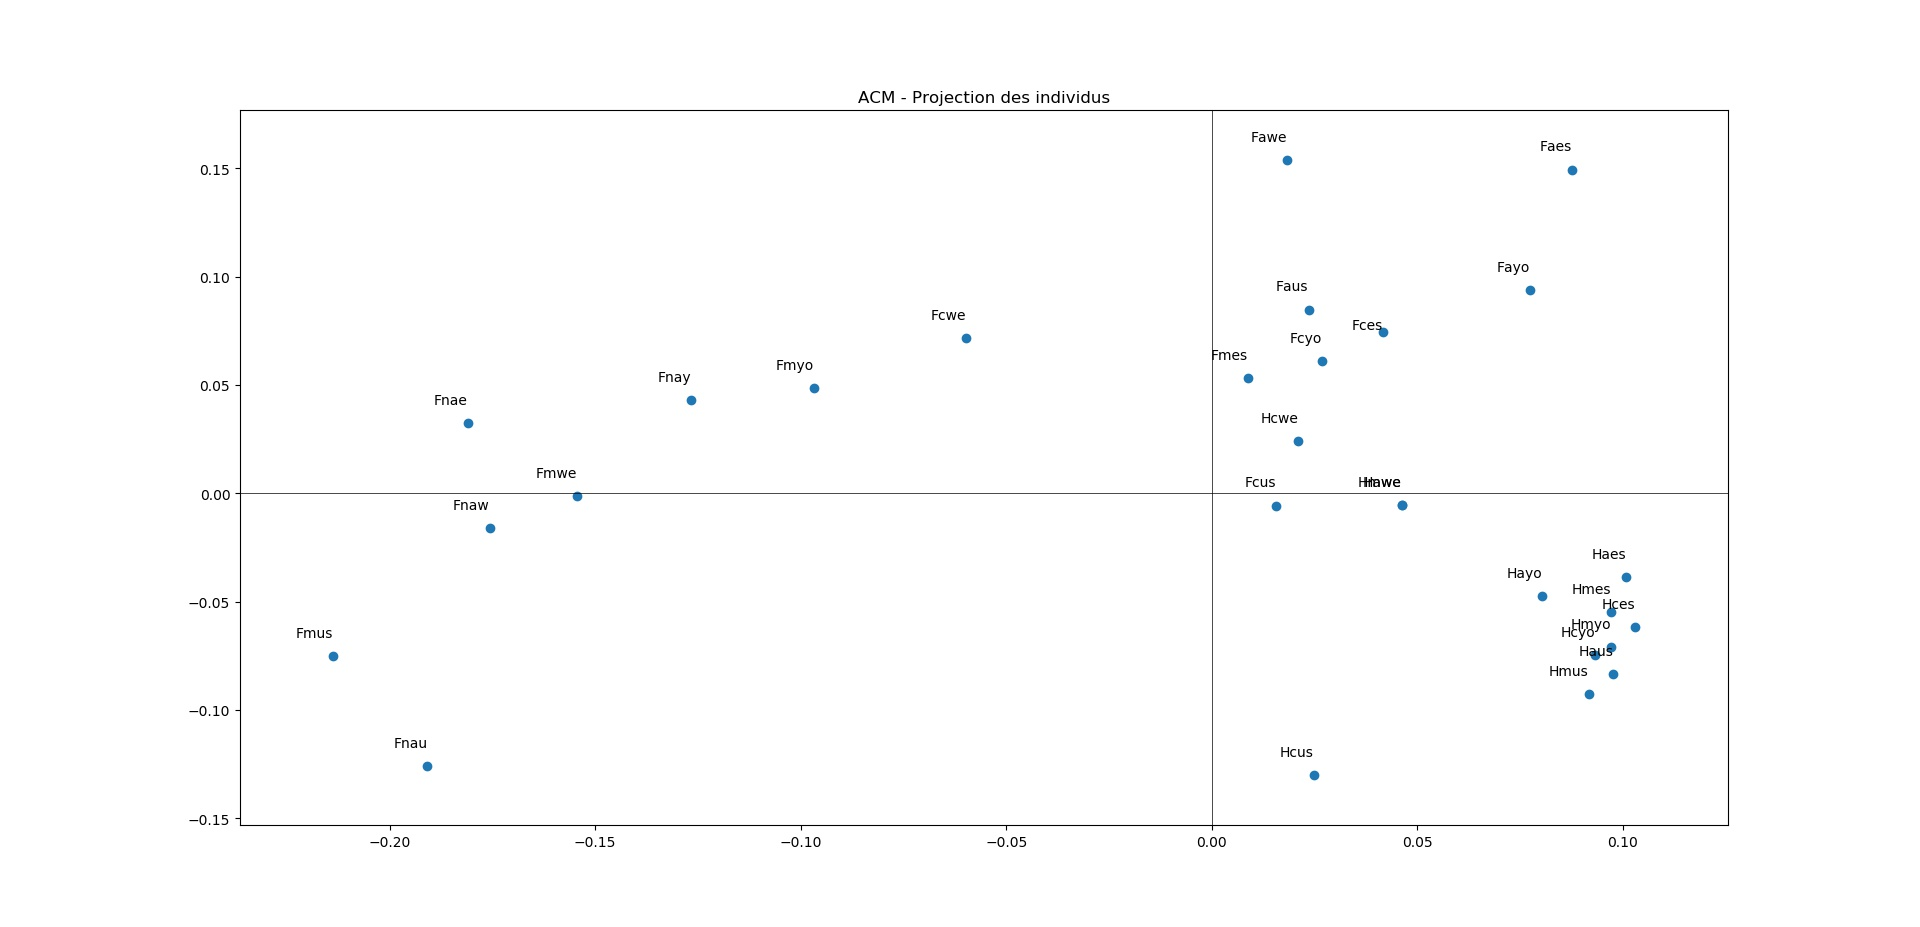
\includegraphics[width=1.0\textwidth]{img/mixte_acm_cah/ACM-Projection_des_individus.jpg}
            \caption{ACM : Projection des individus}
            \label{Label_ACM-Projection_des_individu.jpg}
        \end{subfigure}
        \\
        \begin{subfigure}[b]{1.0\textwidth}
            \centering
            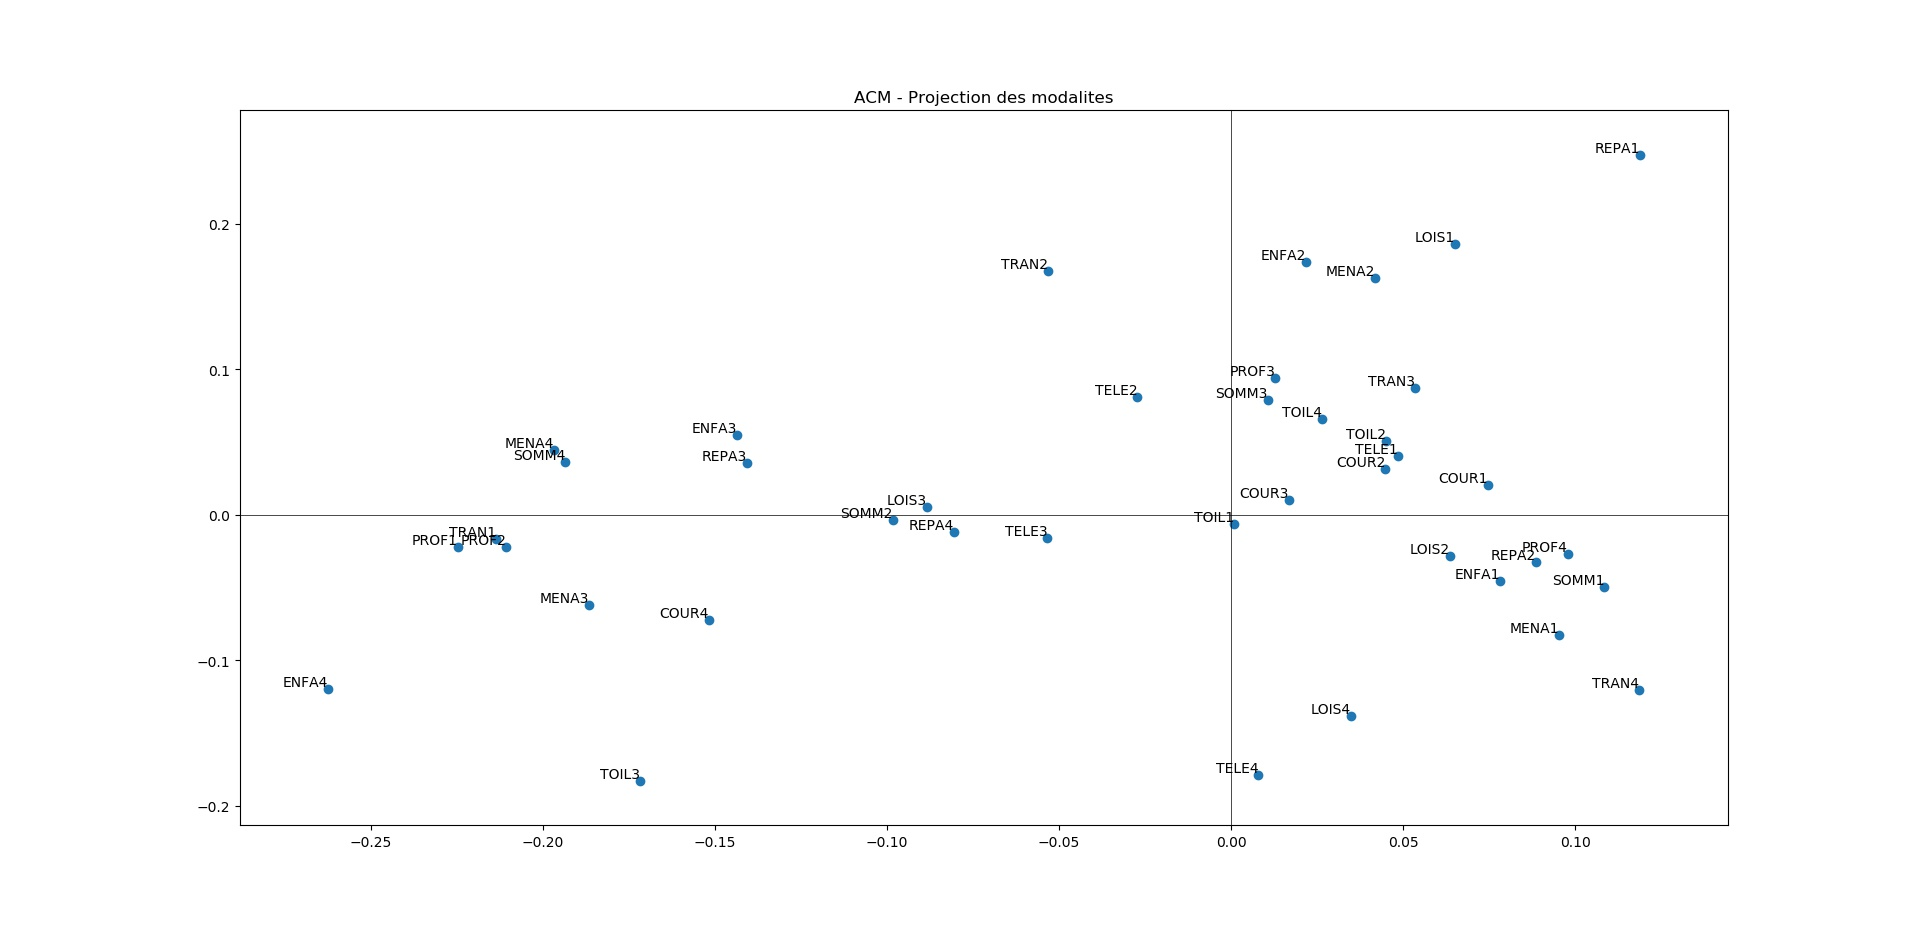
\includegraphics[width=0.9\textwidth]{img/mixte_acm_cah/ACM-Projection_des_modalites.jpg}
            \caption{ACM : Projection des modalités}
            \label{Label_ACM-Projection_des_modalites.jpg}
        \end{subfigure}
        \caption{Projection dans le premier plan factoriel pour l'ACM : individus et variables}
        \label{Label_ACM_Projection_Individus_Modalites.png}
    \end{figure}
    
Les projections des individus et des modalités dans le premier plan factoriel sont montrées dans les Figure \ref{fig: Label_ACM-Projection_des_individu.jpg} et Figure \ref{fig: ACM-Projection_des_modalites.jpg}, respectivement. 
    
Les résultats de la CAH sont affichés ci-dessous. On remarque le fait qu'elle mettre en évidence des classes, mais qui cela a un influence de la méthode choisi.
    
Pour les individus :
    
    \begin{figure}[!htb]
        %\captionsetup[subfigure]{labelformat=empty}
        \begin{subfigure}[b]{1.0\textwidth}
            \centering
            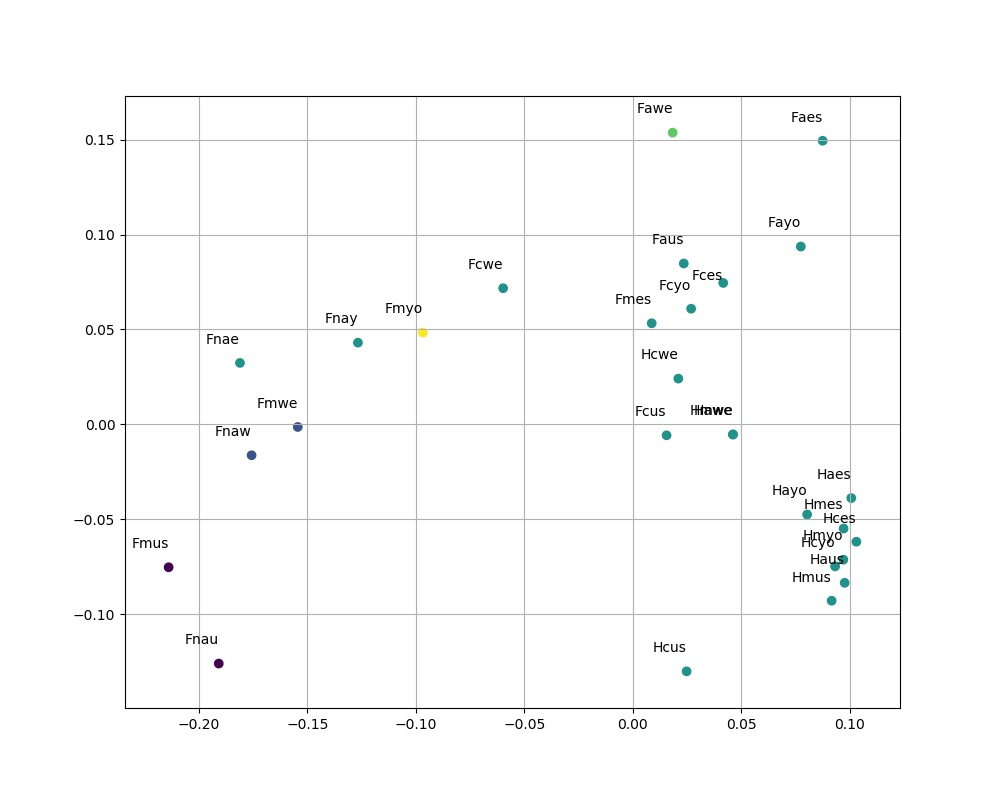
\includegraphics[width=0.78\textwidth]{img/mixte_acm_cah/ACM-Projection_des_individus_cah_'single'_'maxclust'.jpg}
            \caption{ACM + CAH (méthodes single (linkage) et maxclust (fcluster))}
            \label{Label_ACM-Projection_des_individus_cah_'single'_'maxclust'.jpg}
        \end{subfigure}
        \\
        \begin{subfigure}[b]{1.0\textwidth}
            \centering
            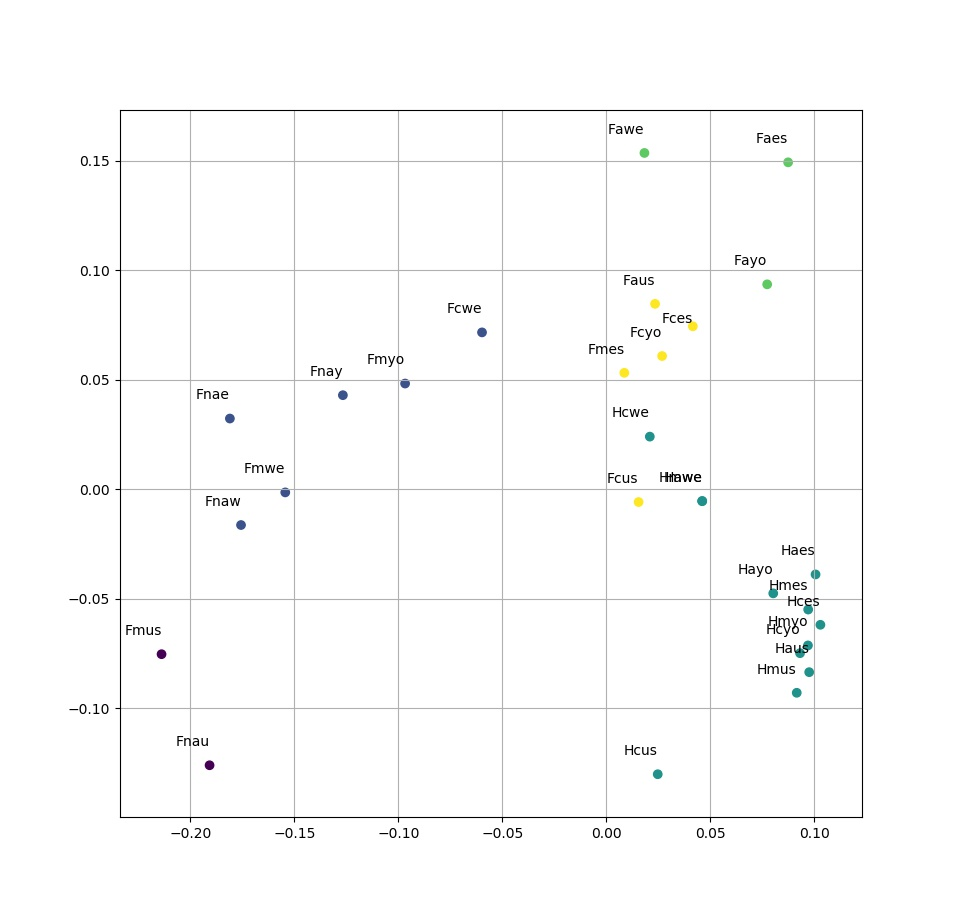
\includegraphics[width=0.78\textwidth]{img/mixte_acm_cah/ACM-Projection_des_individus_cah_'ward'_'maxclust'.jpg}
            \caption{ACM + CAH (méthodes ward (linkage) et maxclust (fcluster))}
            \label{ACM-Projection_des_individus_cah_'ward'_'maxclust'.jpg}
        \end{subfigure}
        \caption{Comparaison ACM + CAH : single x ward pour les individus}
        % \label{Label_ACM_Projection_Individus_Variables.png}
    \end{figure}
    
    \begin{figure}[!htb]
        %\captionsetup[subfigure]{labelformat=empty}
        \begin{subfigure}[b]{1.0\textwidth}
            \centering
            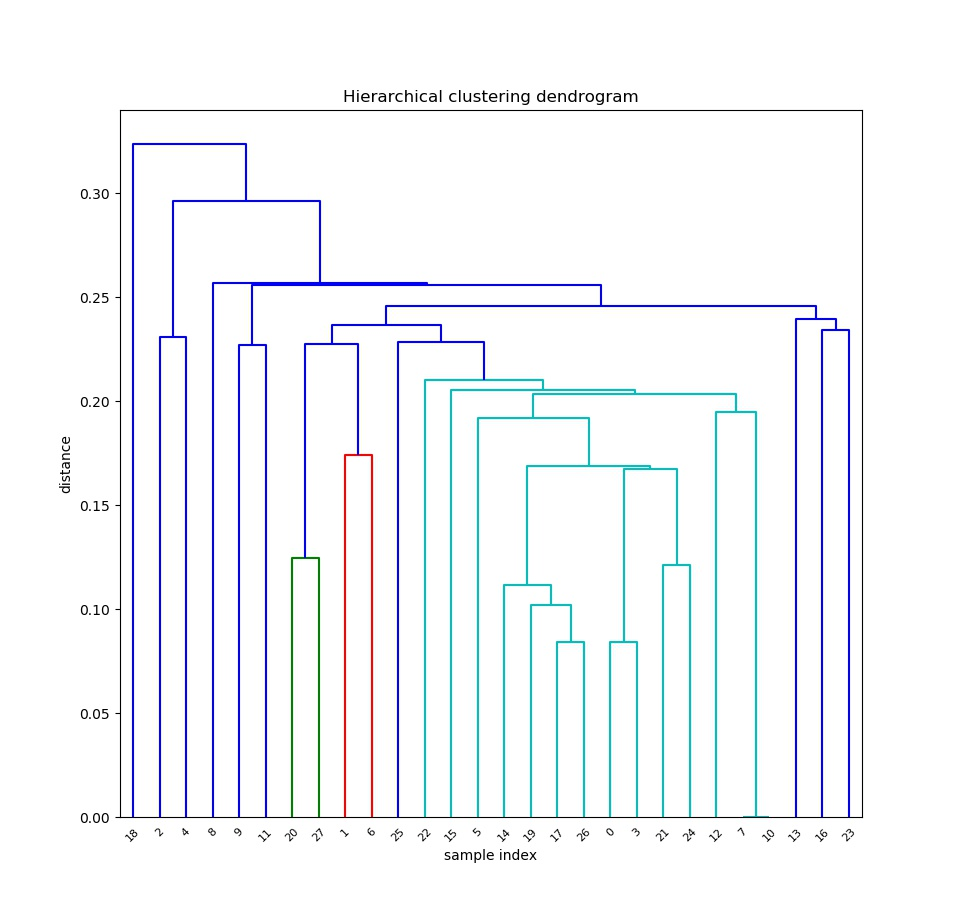
\includegraphics[width=0.71\textwidth]{img/mixte_acm_cah/Dendrogram_individus_'single'_'maxclust'.jpg}
            \caption{Individus : ACM + CAH (méthodes single (linkage) et maxclust (fcluster))}
            \label{Label_ACM_Dendrogram_individus_'single'_'maxclust'.jpg}
        \end{subfigure}
        \\
        \begin{subfigure}[b]{1.0\textwidth}
            \centering
            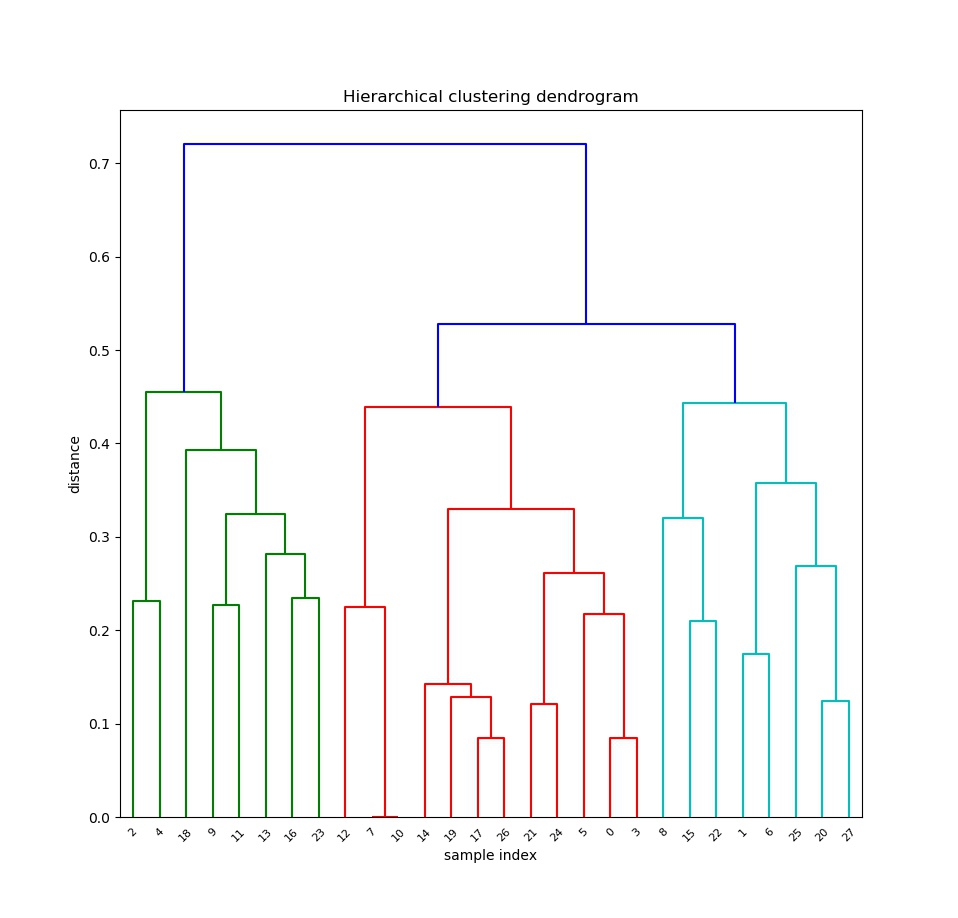
\includegraphics[width=0.71\textwidth]{img/mixte_acm_cah/Dendrogram_individus_'ward'_'maxclust'.jpg}
            \caption{Individus : ACM + CAH (méthodes ward (linkage) et maxclust (fcluster))}
            \label{Label_ACM_Dendrogram_individus_'ward'_'maxclust'.jpg}
        \end{subfigure}
        \caption{Comparaison Dendrograms ACM + CAH : single x ward pour les individus}
        % \label{Label_ACM_Projection_Individus_Variables.png}
    \end{figure}
    
    Pour les modalités :
    
    \begin{figure}[!htb]
        %\captionsetup[subfigure]{labelformat=empty}
        \begin{subfigure}[b]{1.0\textwidth}
            \centering
            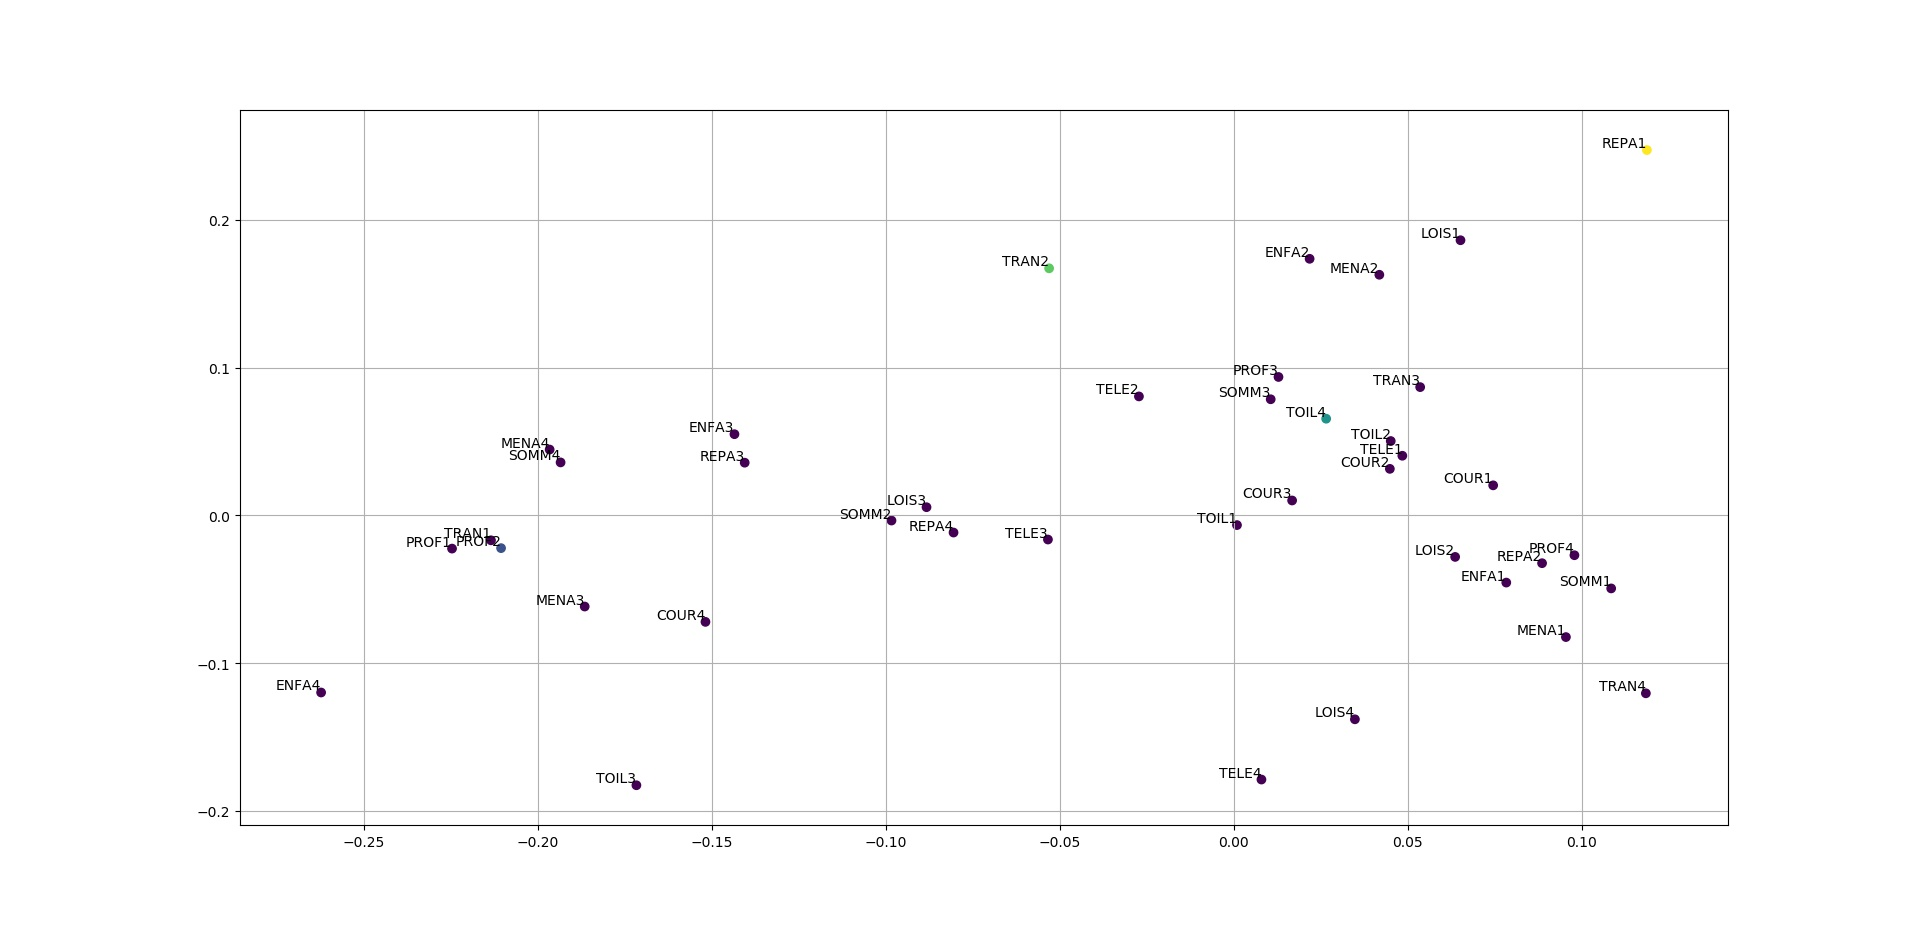
\includegraphics[width=1.0\textwidth]{img/mixte_acm_cah/ACM-Projection_des_modalites_cah_'single'_'maxclust'.jpg}
            \caption{Modalités : ACM + CAH (méthodes single (linkage) et maxclust (fcluster))}
            \label{Label_ACM-Projection_des_modalites_cah_'single'_'maxclust'.jpg}
        \end{subfigure}
        \\
        \begin{subfigure}[b]{0.6\textwidth}
            \centering
            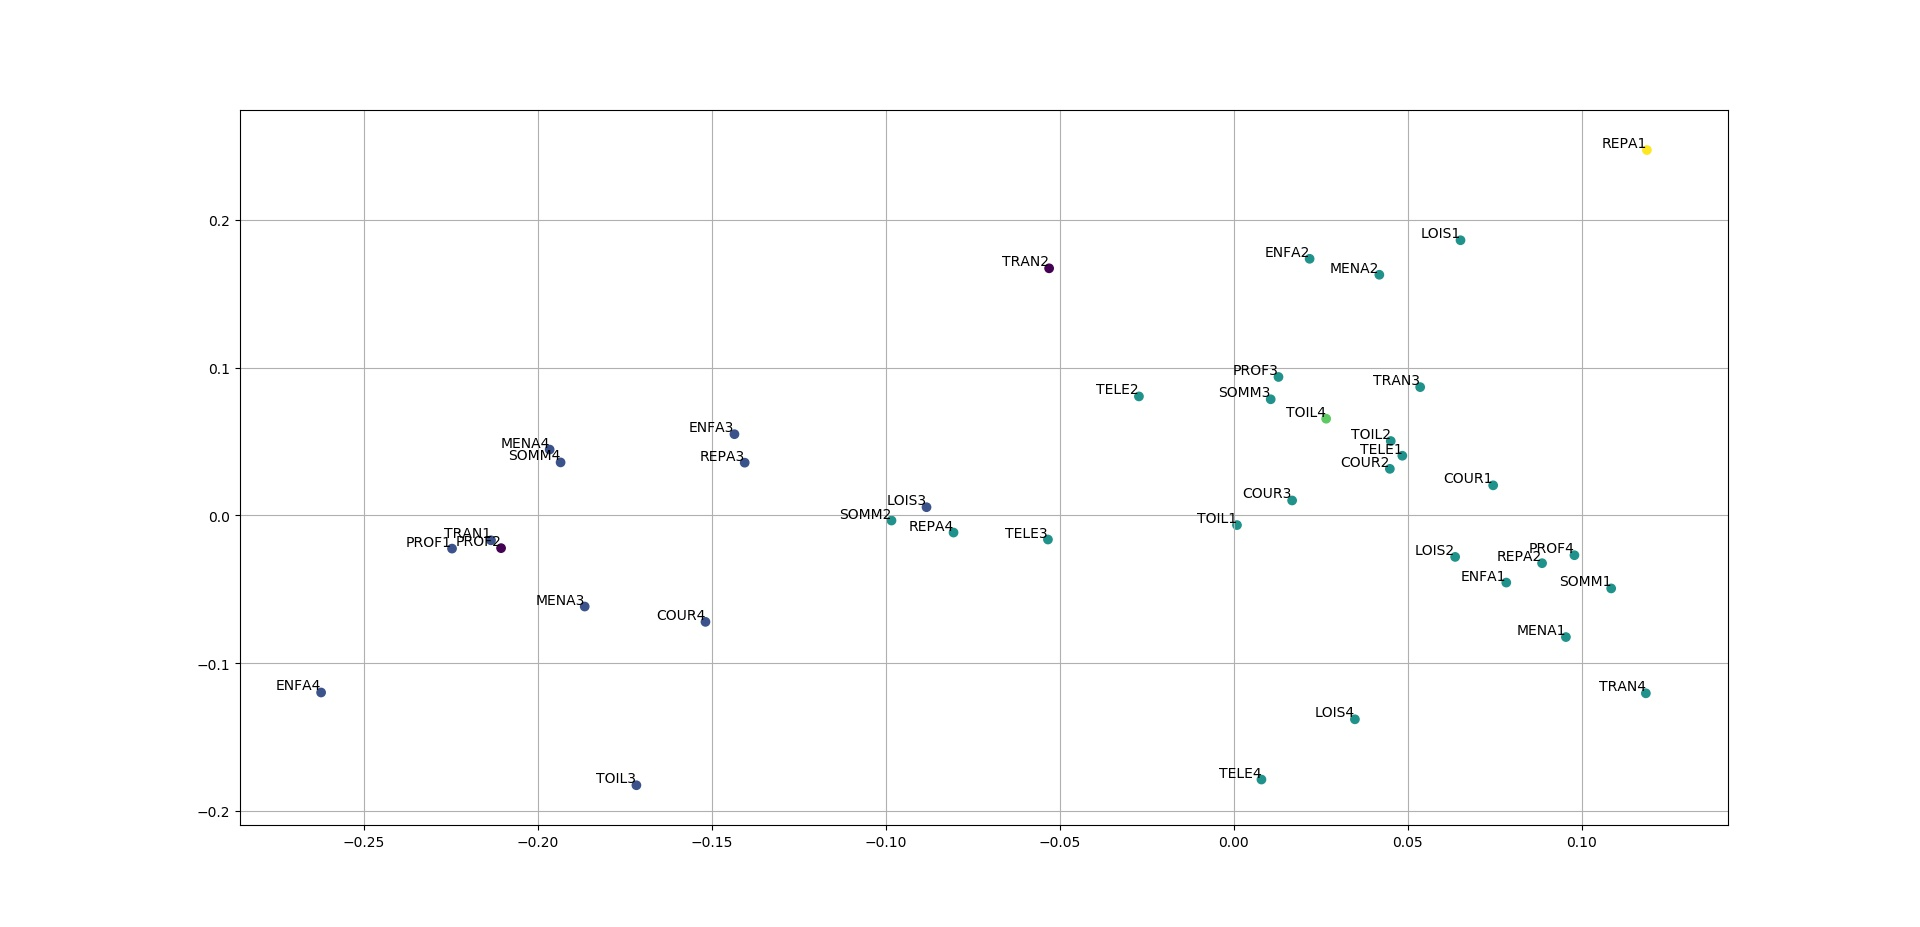
\includegraphics[width=1.0\textwidth]{img/mixte_acm_cah/ACM-Projection_des_modalites_cah_'ward'_'maxclust'.jpg}
            \caption{Modalités : ACM + CAH (méthodes ward (linkage) et maxclust (fcluster))}
            \label{Label_ACM-Projection_des_modalites_cah_'ward'_'maxclust'.jpg}
        \end{subfigure}
        \caption{Comparaison ACM + CAH : single x ward pour les modalités}
        % \label{Label_ACM_Projection_Individus_Variables.png}
    \end{figure}
    
    \begin{figure}[!htb]
        %\captionsetup[subfigure]{labelformat=empty}
        \begin{subfigure}[b]{1.0\textwidth}
            \centering
            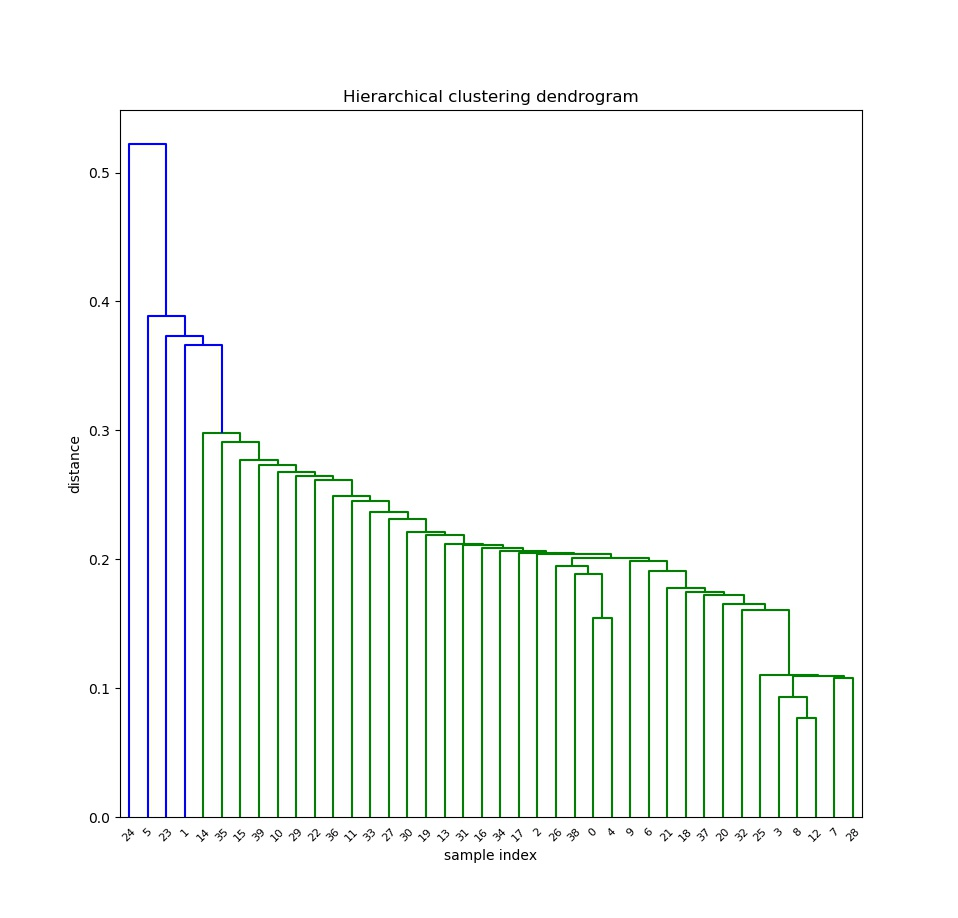
\includegraphics[width=0.7\textwidth]{img/mixte_acm_cah/Dendrogram_modalites_'single'_'maxclust'.jpg}
            \caption{Modalités : ACM + CAH (méthodes single (linkage) et maxclust (fcluster))}
            \label{Label_Dendrogram_modalites_'single'_'maxclust'.jpg}
        \end{subfigure}
        \\
        \begin{subfigure}[b]{1.0\textwidth}
            \centering
            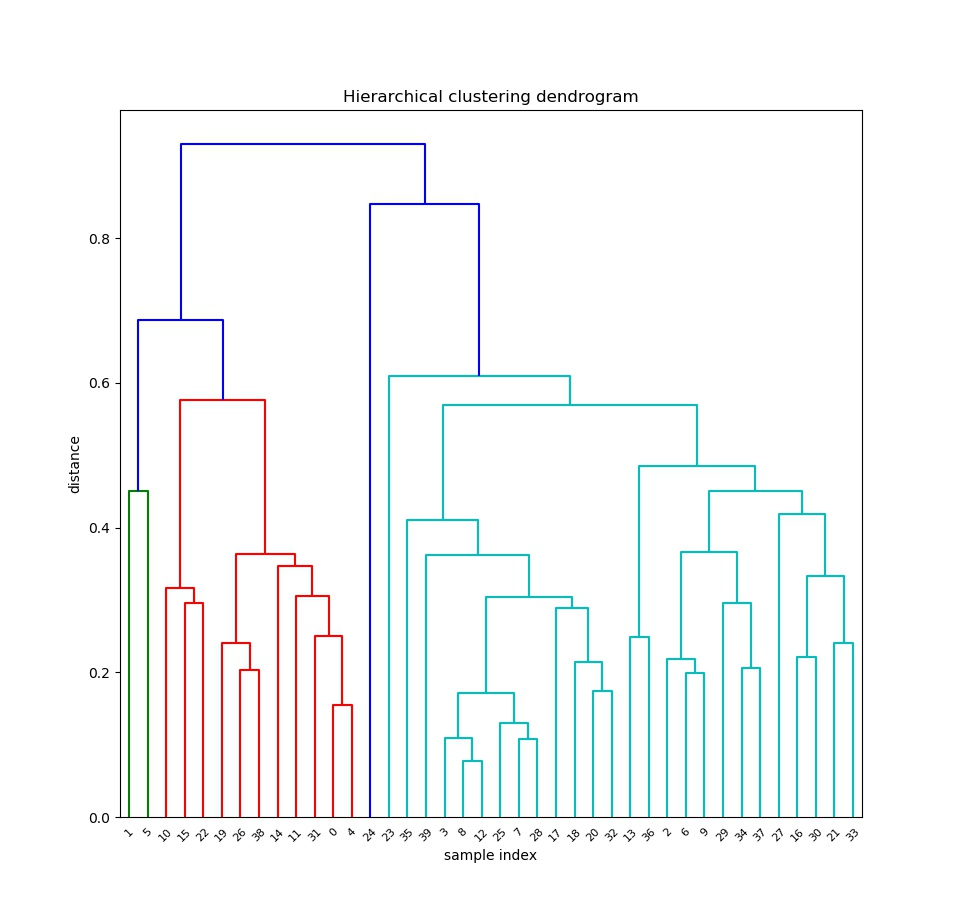
\includegraphics[width=0.7\textwidth]{img/mixte_acm_cah/Dendrogram_modalites_'ward'_'maxclust'.jpg}
            \caption{Modalités : ACM + CAH (méthodes ward (linkage) et maxclust (fcluster))}
            \label{Label_Dendrogram_modalites_'ward'_'maxclust'.jpg}
        \end{subfigure}
        \caption{Comparaison Dendrograms ACM + CAH : single x ward pour les variables}
        % \label{Label_ACM_Projection_Individus_Variables.png}
    \end{figure}


\subsubsection{Commentaires et interprétation}


On a observé ci dessus une classification satisfaisante des éléments. Cela permet dans l'exemple de données traité, de regrouper les métiers et occupations des individus en fonction du temps que cela leur prend, par exemple.

On remarque la coïncidence de quelques points pour l'ACM + CAH. Cela vient du fait de les individus sont dans la même classe pour la mise en classes choisi. 